\section{Characteristics in industrial environments}
\label{characteristics_in_industrial_environments}
An investigation of an representative industrial area where mobile robots are used, shows that areas share common dynamical characteristics. Parts of the production line at SCAN A/S, where a MIR robot is used, are shown in figure \ref{fig:scan-mir} and \ref{fig:scan-semi-static-obstacles}.

\begin{table}[htbp]
	\caption{Regions of industrial environments}
	\label{tab:regions_of_industrial_environments}
	\begin{center}
		\begin{tabular}{p{2.cm} | p{2.6cm} | p{2.6cm} | p{2.6cm} | p{2.6cm}}
			\toprule
			\textbf{Type} & \textbf{Dominated areas} & \textbf{Object types} & \textbf{In navigation} & \textbf{In localization} \\ 
			\rowcolor[gray]{0.925}
			\textit{Highly dynamic} & Central corridors & Humans, moving vehicles & Avoid these areas if convenient & Consider avoiding this area \\

			\textit{Semi-static} & Temporary Storage areas & Pallets with parts or products & Incorporate for next planning with non-lethal & Landmarks value based on degree of dynamics \\ 
			\rowcolor[gray]{0.925}
			\textit{Static} & The rest & Walls, heavy machinery & Incorporate in map with lethal & Very good landmark \\			
			\bottomrule
		\end{tabular} 
	\end{center}
\end{table}

The areas can roughly be classified based on dynamics of the obstacles that are usually contained within them, as shown in table \ref{tab:regions_of_industrial_environments}. Areas with objects that moves almost constantly like humans are categorized as \textit{highly dynamic}, whereas areas with objects like walls, that never move are categorized as \textit{static}. The remaining \textit{semi-static} objects can be everything from parked vehicles to stored production parts, that moves with minutes or weeks in between. 

\begin{figure}[htbp]
	\centering
	\begin{subfigure}[t]{0.6\textwidth}
		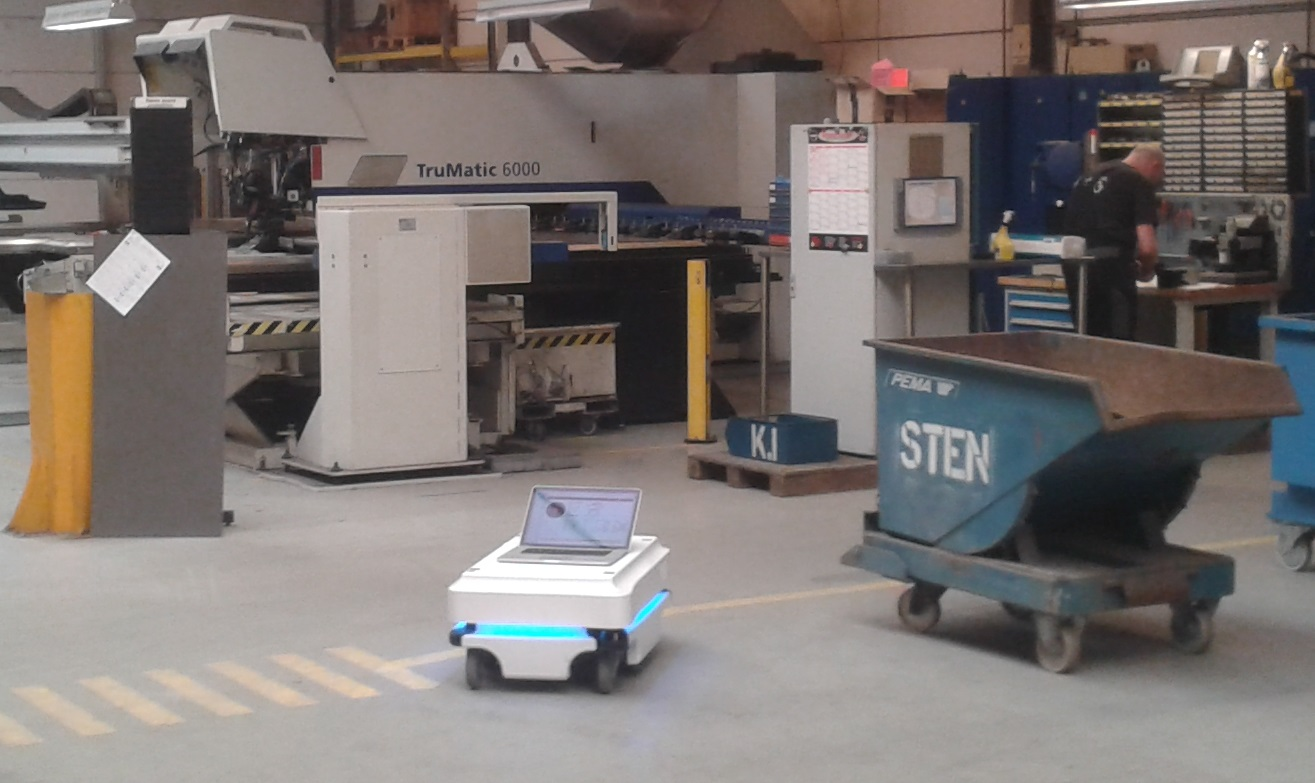
\includegraphics[width=1.0\textwidth]{chapters/mapping_of_dynamic_areas/figures/scan-mir}	
		\caption{MIR 100 robot navigating close to heavy machinery.}
		\label{fig:scan-mir}
	\end{subfigure}
	\begin{subfigure}[t]{0.3875\textwidth}
		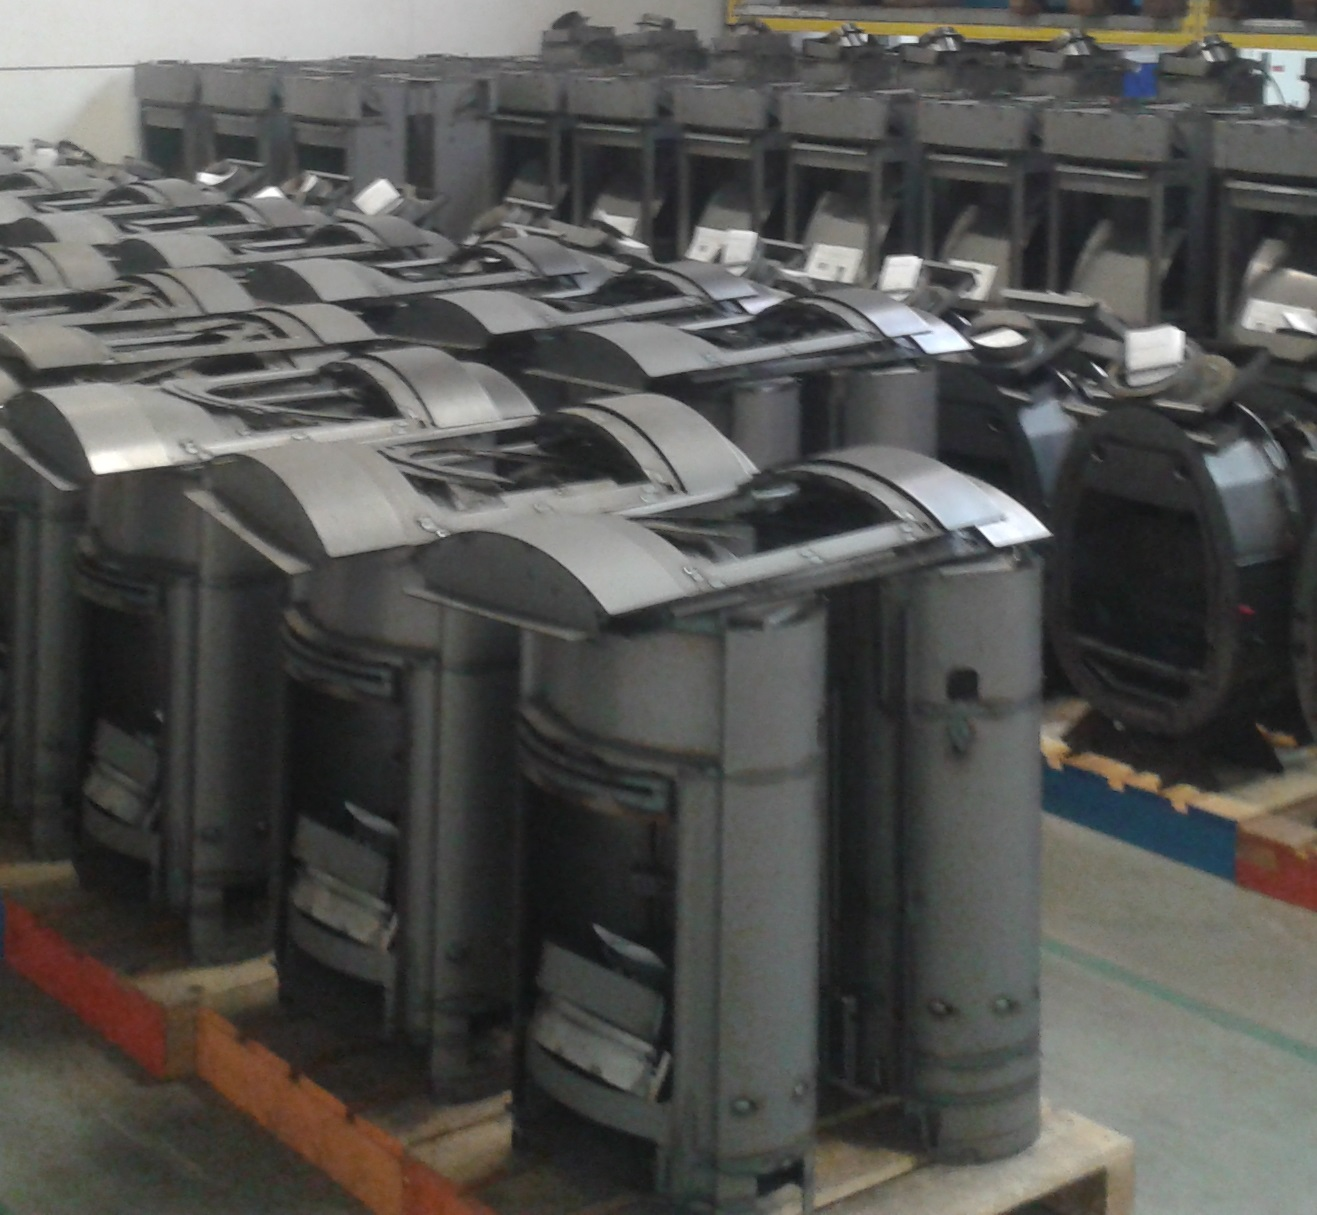
\includegraphics[width=1.0\textwidth]{chapters/mapping_of_dynamic_areas/figures/scan-semi-static-obstacles}
		\caption{\textit{Semi-static} obstacles in the form of product parts.}
		\label{fig:scan-semi-static-obstacles}
	\end{subfigure}
	\caption{Examples of obstacles in the production area at SCAN A/S.}
\end{figure}

The information of these areas can be incorporated in the representation of the world to avoid having to re-plan a path and to improve localization. 

The \textit{highly dynamic} objects should not be considered as landmarks or obstacles, but some re-planning of the plan might. It is beneficial to include \textit{semi-static} obstacles in path planning to avoid having to re-plan, but by assigning them as lethal obstacles it might be impossible to plan a path although one is possible. The \textit{static} objects should always be present as lethal obstacles when path planning to avoid navigating obscure ways.

The \textit{highly dynamic} objects should not be included as landmarks for the localization, since they are moving almost constantly. Since the value of the \textit{semi-static} obstacles as landmarks depends on how dynamic they are, they should be weighted in the localization algorithm accordingly. The \textit{static} obstacles are very good landmarks.